\documentclass{article}
    % General document formatting
    \usepackage[margin=0.7in]{geometry}
    \usepackage[parfill]{parskip}
    \usepackage[utf8]{inputenc}
    
    % Related to math
    \usepackage{amsmath,amssymb,amsfonts,amsthm}
\usepackage{graphicx}
%\usepackage{subfig}
%\usepackage{subfigure}
\usepackage{caption}
\usepackage{subcaption}
\usepackage{listings}
\usepackage{braket}
\usepackage{gensymb}

\usepackage{titling}
%\usepackage{lipsum}

\usepackage{titlesec}

\titleformat*{\section}{\Large\bfseries}
\titleformat*{\subsection}{\large\bfseries}
%\titleformat*{\subsubsection}{\large\bfseries}
%\titleformat*{\paragraph}{\large\bfseries}
%\titleformat*{\subparagraph}{\large\bfseries}
\titlespacing\section{0pt}{12pt plus 4pt minus 2pt}{0pt plus 2pt minus 2pt}
\titlespacing\subsection{0pt}{12pt plus 4pt minus 2pt}{0pt plus 2pt minus 2pt}
\titlespacing\subsubsection{0pt}{12pt plus 4pt minus 2pt}{0pt plus 2pt minus 2pt}

\pretitle{\begin{center}\large\bfseries}
\posttitle{\par\end{center}\vskip 0.01em}
\preauthor{\begin{center}\Large\ttfamily}
\postauthor{\end{center}}
\predate{\par\normalsize\centering}
\postdate{\par}

\title{Population Genetic Analyses of Genomic Data 1}
%\date{\today}


\begin{document}

%\maketitle

\begin{center}
\textbf{\LARGE{\centering{Computational Neuroscience 2}}}\\

\textit{USN: 303039534}\\
\end{center}

%\normalsize{   }

\section{Unsupervised learning}

For a general many-input-one-output network we can define an input vector \textbf{u} as the activity of the neurons in the input layer and a weight vector \textbf{w} as the strength of connections between the input neurons and the output neuron. The total input to the output neuron is thus.
\begin{equation}
v = \bf{w} \cdot \bf{u} 
\end{equation}

Based on Hebb's conjecture from 1949, we can write a simple learning rule where the strength of a synapse increases with pre- and post-synaptic coactivity:
\begin{equation}
\tau_w \dfrac{d\bf{w}}{dt} = v \bf{u}
\end{equation}

If we assume that synaptic weight changes occur over a much slower timescale than the inputs, we can use 'batch learning' and average over all input data in every learning step:
\begin{equation}
\tau_w \dfrac{d\bf{w}}{dt} = \braket{v \bf{u}}
\end{equation}
Since $v = \bf{w} \cdot \bf{u} $ and defining the correlation matrix ${\bf Q} = \braket{{\bf u u} }$, this allows us to learn weights using simple matrix multiplication
\begin{equation}\label{eq:batchlearn}
\tau_w \dfrac{d\bf{w}}{dt} = \bf Q \cdot w
\end{equation}
Note that this definition of 'correlation' is slightly odd, as for example the self correlation is given by $Q_{ii} = \braket{u_i^2}$ rather than self correlations always being 1.
We then continue to iterate over equation \ref{eq:batchlearn} until the weights have converged. If the activity of our neurons corresponds to firing rates, all $u_i$ must be positive. The correlation matrix is therefore a non-negative matrix and we cannot learn negative correlations. Instead, it is therefore common to use a covariance-based learning rule where we let $\bf u' = u-\braket{u}$. Now defining the covariance matrix ${\bf C} = \braket{( {\bf u} - \braket{\bf u})  ( {\bf u} - \braket{\bf u})}$ we can rewrite our learning rule as
\begin{equation}\label{eq:cov}
\tau_w \dfrac{d\bf{w}}{dt} = \bf C \cdot w
\end{equation}
We note that since these batch learning rules are linear in \textbf{w}, we can treat them analytically.
At any given time, we can decompose the weight vector in terms of the eigenvectors $e_\mu$ of \textbf{C}:
\begin{equation}
{\bf w}(t) = \sum_\mu{ c_\mu(t) {\bf e}_\mu }
\end{equation}
Solving the linear differential equation \ref{eq:cov} we get
\begin{equation}
c_\mu = \exp{( \dfrac{\lambda_\mu t}{\tau_w})}({\bf w}(0) \cdot {\bf e_\mu})
\end{equation}
Putting these results together gives
\begin{equation}\label{eq:anal}
{\bf w}(t) = \sum_\mu{ \exp{( \dfrac{\lambda_\mu t}{\tau_w})}({\bf w}(0) \cdot {\bf e_\mu})  {\bf e}_\mu}
\end{equation}
If the covariance matrix is non-degenerate, we expect the eigenvector corresponding to the highest eigenvalue to dominate this sum at long times due to the coefficient being exponential in the eigenvalue. This in turn suggests that the weight vector will converge towards this first principal component unless it is orthogonal to the initial weight matrix.
However, this basic Hebbian learning will lead to unphysiological unbounded weight increases and is therefore usually augmented with some sort of normalization which can alter the simple behavior expected from equation \ref{eq:anal} as will be evident from the next two sections.

We note that since the timescale is arbitrary for the above equations, we can set $\tau_w = 1$ for the remainder of this section without loss of generality. We require dt to be smaller than $\tau_w$ for accurate Euler integration and therefore let dt=0.01. This is equivalent to using a discrete learning rule with $\epsilon = \dfrac{dt}{\tau_w}=0.1$.

\subsection{Multiplicative normalization}

One commonly used form of normalization is multiplicative normalization where we subtract a term from the simple Hebbian learning rule proportional to the current weights at each iteration. We implement this using Oja's learning rule:
\begin{equation}\label{eq:ojacont}
\tau_w \dfrac{d\bf{w}}{dt} = v {\bf{u}} - \alpha v^2 {\bf{w}}
\end{equation}
To see how this leads to normalization, we take the dot product of equation \ref{eq:ojacont} with \textbf{w}
\begin{equation}
\tau_w \dfrac{d|{\bf{w}}|^2}{dt} = v {\bf{w} \cdot \bf{u}} - \alpha v^2 {\bf{w} \cdot \bf{w}} = v^2(1-\alpha |{\bf{w}}|^2)
\end{equation}
Hence $\dfrac{d|{\bf{w}}|^2}{dt} \rightarrow 0$ as $\alpha |{\bf{w}}|^2 \rightarrow 1$ and Oja normalization constrains the modulus of the weight vector. At long times, we thus converge towards a weight vector of magnitude $|{\bf{w}}| \rightarrow \dfrac{1}{\sqrt{\alpha}}$. In the following, we let $\alpha=1$ such that the weight vector converged to is normalized.

As above, we average over the training inputs and get a batch learning rule
\begin{equation}\label{eq:oja}
\tau_w \dfrac{d\bf{w}}{dt} = {\bf Q \cdot w} - \alpha ({\bf w \cdot Q \cdot w}) {\bf w}
\end{equation}
We then update weights according to equation \ref{eq:oja} until the norm of the change in weights between iterations is $\epsilon < 10^{-6}$. Setting $\alpha=1$ we note that when \textbf{w} becomes an eigenvector of \textbf{Q} with eigenvalue $\lambda$, we can write ${\bf Q \cdot w} = \lambda \bf w$ and $({\bf w \cdot Q \cdot w}) = \lambda$, giving  $\tau_w \dfrac{d\bf{w}}{dt} =0$. For Oja's rule, we thus expect the weight vector to converge to an eigenvector of \textbf{Q}, and we expect this to be the largest eigenvector on the basis of equation \ref{eq:anal}.

We see an example of this in figure \ref{fig:sim1mul} where we train the network on a two-dimensional Gaussian dataset with each point corresponding to a two-dimensional input datapoint \textbf{u}. The red line indicates the direction of the final weight vector, shifted vertically to run through the mean of the dataset, and we see that it does indeed align with the first principal component (the axis of maximum variability).

However, if we shift the mean of the gaussian input dataset to (3,3), the correlation matrix \textbf{Q} becomes a positive matrix and the largest eigenvalue now corresponds to the eigenvector (1,1) although there is still a negative covariance between the x and y component of the data (figure \ref{fig:sim2mul}). In this case, the converged weight vector thus ends up being perpendicular to the first principal component of the data.

However, we can salvage this behavior by using the covariance-based learning rule from equation \ref{eq:cov} on the same dataset (figure \ref{fig:sim3mul}). This allows us to once again capture the negative covariance between the components $u_1 \& u_2$ as the converged weight vector aligns with the first principal component of the data.

\begin{figure}[h]
	\centering
	\begin{subfigure}[t]{0.30\linewidth}
		\centering
		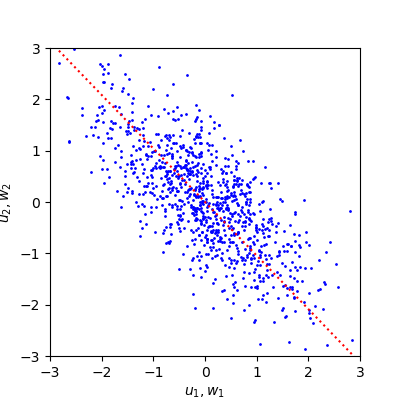
\includegraphics[width = 1.0\linewidth, trim={0 0 0 0}, clip=true]{figures/2d_sim1.png}
		\subcaption{Mean (0,0) with correlation-based training. Final weight vector: [0.692, -0.722], principal components: [-0.692, 0.722] \& [-0.722, -0.692]}
		\label{fig:sim1mul}	
	\end{subfigure}%
	\hspace{0.03\linewidth}
	\begin{subfigure}[t]{0.30\linewidth}
		\centering
		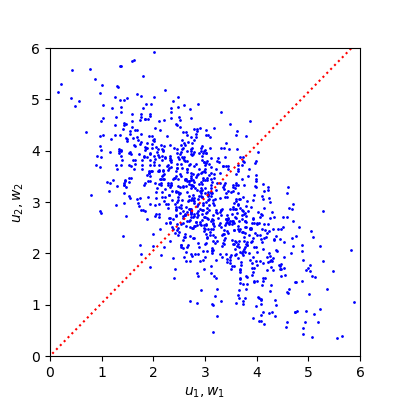
\includegraphics[width = 1.0\linewidth, trim={0 0 0 0}, clip=true]{figures/2d_sim2.png}
		\subcaption{Mean (3,3) with correlation-based training. Final weight vector [-0.697, -0.717], principal components[-0.692, 0.722] [-0.722, -0.692]}
		\label{fig:sim2mul}	
	\end{subfigure}%
	\hspace{0.03\linewidth}
	\begin{subfigure}[t]{0.30\linewidth}
		\centering
		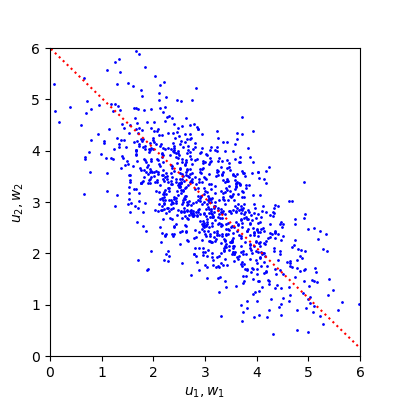
\includegraphics[width = 1.0\linewidth, trim={0 0 0 0}, clip=true]{figures/2d_sim3.png}
		\subcaption{Mean (0,0) with covariance-based training. Final weight vector [0.716, -0.698], principal components [-0.716, 0.698] [-0.698, -0.716]}
		\label{fig:sim3mul}	
	\end{subfigure}%
\caption{Learning weight vectors from 500 input data points with Oja's rule. In each case, we start from [w1, w2] = [0.001, 0.001] and iterate through equation \ref{eq:oja} until convergence using either a correlation or covariance-based learning rule. Red dotted lines indicate the direction of the final weight vector. All datasets were generated with a standard deviation of 1 and $1-\rho^2$ in the $u1$ and $u2$ directions and a correlation of $\rho = -0.7$.}
\label{fig:multiplicative}
\end{figure}

If instead we were to have a positive covariance between the u1 and u2 components of our input vectors, the final weight vector aligns with the principal component irrespective of whether the mean of our distribution is zero, positive or negative provided the mean of both the u1 and u2 components have the same sign. In this case we instead fail to recover the first principal component in the case where the mean of the u1 is positive while the mean of u2 is negative or vice versa. In that case we get a final vec of [0.692383, -0.72153] despite a principal component of [0.688815, 0.724937]. This is again salvaged by using a covariance-based learning rule.

We can also investigate the magnitude of our weight vectors over time since we expect these to converge smoothly to 1 as discussed above, and we see that this is indeed the case (figure \ref{fig:multiplicativevec}). Interestingly, it appears that convergence to the [1,1] vector in our second simulation is much faster than converging to a [-1, -1] vector in the first and third simulations.

\begin{figure}[h]
	\centering
	\begin{subfigure}[t]{0.30\linewidth}
		\centering
		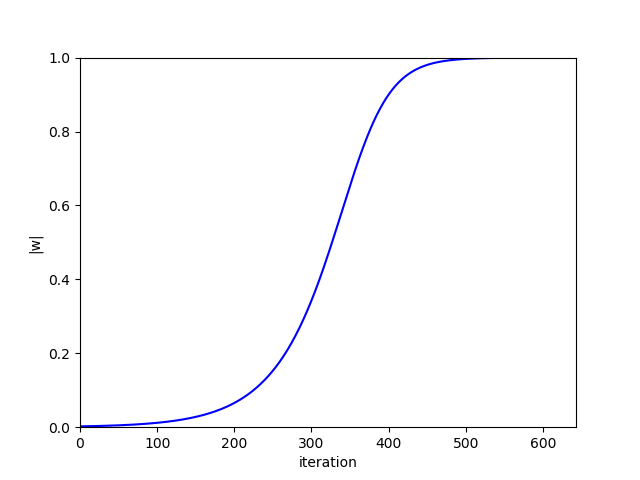
\includegraphics[width = 1.0\linewidth, trim={0 0 0 0}, clip=true]{figures/2d_sim1_vec.png}
		\subcaption{}
		\label{fig:sim1vec}	
	\end{subfigure}%
	\hspace{0.03\linewidth}
	\begin{subfigure}[t]{0.30\linewidth}
		\centering
		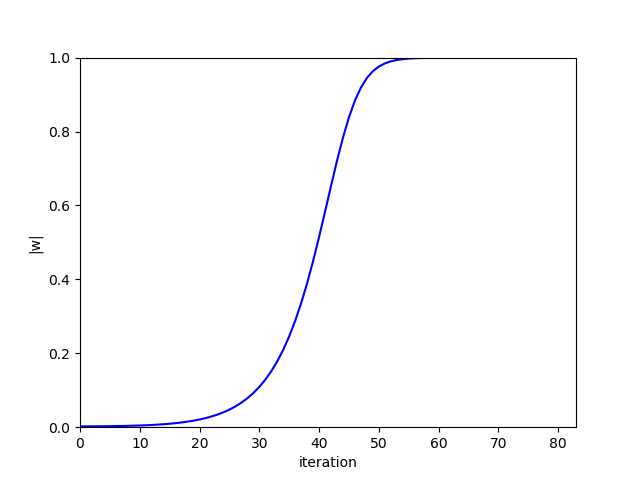
\includegraphics[width = 1.0\linewidth, trim={0 0 0 0}, clip=true]{figures/2d_sim2_vec.png}
		\subcaption{}
		\label{fig:sim2vec}	
	\end{subfigure}%
	\hspace{0.03\linewidth}
	\begin{subfigure}[t]{0.30\linewidth}
		\centering
		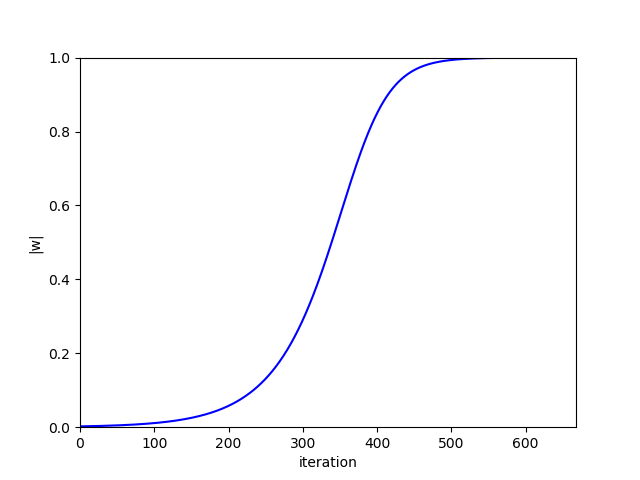
\includegraphics[width = 1.0\linewidth, trim={0 0 0 0}, clip=true]{figures/2d_sim3_vec.png}
		\subcaption{}
		\label{fig:sim3vec}	
	\end{subfigure}%
\caption{Weight vector magnitue as a function of iteration number for the three simulations in figure \ref{fig:multiplictive}}
\label{fig:multiplicativevec}
\end{figure}

\subsection{Subtractive normalization}

A different form of normalization that is commonly used to prevent excessive growth of weights is subtractive normalization as specified in equation \ref{eq:subcont}.

\begin{equation}\label{eq:subcont}
\tau_w \dfrac{d\bf{w}}{dt} = v {\bf{u}} - \dfrac{v(\bf{n}\cdot {\bf{u}}) {\bf{n}}}{N_u}
\end{equation}
This constrains the sum of the weights to be constant as can be proven by taking the dot product with \textbf{n} where \textbf{n} is a vector of ones:
\begin{equation}
\tau_w \dfrac{d\bf{n} \cdot \bf{w}}{dt} = \tau_w \dfrac{d\sum_i{w_i}}{dt} = v{\bf{n}} \cdot {\bf{u}}(1 - \dfrac{\bf{n}\cdot {\bf{n}}}{N_u}) = 0
\end{equation}

The total sum of the weights in the system is thus constant, but these weights must still be thresholded to avoid unbounded growth of complementary rates towards $\pm \infty$. This is commonly achieved by constraining all weights to be $\geq 0$ in weight case there is an upper saturation limit of $w_{max} = \sum_i{w_i(0)}$.

We once again average our learning rule from equation \ref{eq:subcont} over the training data and get

\begin{equation}\label{eq:subavg}
\tau_w \dfrac{d\bf{w}}{dt} = {\bf Q \cdot w} - \dfrac{({\bf w \cdot Q \cdot n}) {\bf n} }{N_u}
\end{equation}

Even using identical initial weights, we will still converge to [0,1] rather than obeying the symmetry of the initial weights, since the data is noisy which leads to our covariance and correlation matrices having non-identical diagonal elements, leading to symmetry breaking. This also makes sense in the context of these learning rules being approximations to learning by presentation of individual datappoints, as we would require every individual datapoint to be symmetric and u1 and u2 to conserve the initial symmetry of the weights.

\Huge{We can of course just set rho to 0 or 1 and get data aligned with the x or y axis!
Also fix diagonal elements and let the initial weight vector be either parallel or perpendicular to the principal components. (p296). try positively and negatively correlated data.}
\normalsize

\section{Ocular dominance columns}

In the following, we consider a many-input-many-ouput recurrent circuit with input vector $\bf u$, feedforward weight matrix $\bf W$ and thus total input vector $\tilde {\bf u} = {\bf W \cdot u}$. We additionally let the system have a fixed recurrent weight matrix $\bf M$. The dynamics of this system follow differential equation \ref{eq:occont}
\begin{equation}\label{eq:occont}
\tau_r \dfrac{d \bf v}{dt} = -{\bf v} + {\bf W \cdot u} + {\bf M\cdot v}
\end{equation}
Provided that the eigenvalues of \textbf{M} have real parts $<1$, a stability analysis shows that this system will have a stable fixed point with steady state activity given by 
\begin{equation}
{\bf v} = {\bf W \cdot u} + {\bf M \cdot v}
\end{equation}
Which has the solution
\begin{equation}
{\bf v} = {\bf K \cdot W \cdot u}
\end{equation}
Where ${\bf K} = ({\bf I} - {\bf M})^{-1}$.

If we now fix the recurrent weights and let the feedforward weights change according to a Hebbian learning rule, the time evolution of the weights is determined by equation \ref{eq:ocheb} with $\bf Q$ defined as in section 1.
\begin{equation}\label{eq:ocheb}
\tau_w \dfrac{d{\bf W}}{dt} = \braket{\bf vu} = {\bf K \cdot W \cdot Q}
\end{equation}
We will use a discretized form of this equation with $\epsilon = 0.01$:
\begin{equation}\label{eq:ocdic}
{\bf W}_{n+1} = {\bf W}_n + \epsilon \bf K W Q
\end{equation}
%Finally we use subtractive normalization as in equation \ref{eq:subavg} which gives
%\begin{equation}
%{\bf W}_{n+1} = {\bf W}_n + \epsilon \bf K W Q - ???
%\end{equation}

We now consider a highly simplified model of ocular dominance including only a single direction along the cortex and a single point in the visual field. This gives rise to only two input activities $u_R$ and $u_L$ corresponding to the input from the right and left eyes. We include 512 output units in the model indexed with the label $a$ which also specifies their location along the 1-dimensional cortex of length $L = 10$mm.
We also assume the cortical interactions specified by $\bf K$ to be translationally invariant and impose periodic boundary conditions requiring $v_0 = v_{512}$ to avoid edge effects.

Assuming that the right and left eye are statistically equivalent, we can now write the input correlation matrix as
\[
{\bf Q} = 
\begin{bmatrix}
   \braket{u_R u_R} & \braket{u_R u_L} \\
   \braket{u_L u_R} & \braket{u_L u_L}  \\
\end{bmatrix}
=
\begin{bmatrix}
   q_S &q_D \\
   q_D & q_S  \\
\end{bmatrix}
\]
Expanding the weight matrix $\bf W$ into its component vectors ${\bf w}_R$ and ${\bf w}_L$, we can consider the in-phase and out-of-phase combination of these vectors ${\bf w}_+ = {\bf w}_R + {\bf w}_L $ and ${\bf w}_- = {\bf w}_R - {\bf w}_L $ seperately. When expanding out equation \ref{eq:ocdic}, these evolve according to
\begin{equation}
{\bf w}_{+}^{n+1} = \epsilon (q_S+q_D){\bf K \cdot w}_+^n
\end{equation}
\begin{equation}
{\bf w}_{-}^{n+1} = \epsilon (q_S-q_D){\bf K \cdot w}_-^n
\end{equation}

Using subtractive normalization for each pair of weights $w_L(a)$ and $w_R(a)$, we can leave ${\bf w}_+$ fixed while ${\bf w}_-$ changes. We therefore consider only ${\bf w}_-$ in the following and investigate how this weight vector changes over time.

Since the growth of ${\bf w}_-$ is proportional to $(q_S-q_D)$, these correlation parameters do not effect the long term behavior of the system but merely the timescale over which it changes provided that $q_D > q_S > 0$. We therefore arbitrarily let $q_S = 1$ and $q_D = 0.7$ for the remainder of this section. 

In the present case, we implement subtractive normalization naively by performing the following update steps at each iteration:
\begin{equation}\label{eq:ocdic2}
{\bf W}_{n+1} = {\bf W}_n + \epsilon \bf K W Q
\end{equation}
\begin{equation}
W_{n+1} = W_{n+1} + 0.5 (1 - \text{rowsum}(W_{n+1}))
\end{equation}
\begin{equation}
W_{n+1}[ W_{n+1} < 0 ] = 0
\end{equation}
\begin{equation}\label{eq:subnorm}
W_{n+1}[ W_{n+1} > 1 ] = 1
\end{equation}

We intialize the weights such that ${\bf w}_L = 0.5 + \epsilon$ and ${\bf w}_R = 1 - {\bf w}_L$ where $\epsilon =  \mathcal{N}(0, 0.01)$. This approach ensures that ${\bf w}_+ = 1$ at all times and implements subtractive normalization with thresholds of 0 and 1. This could have been implemented in a similar way to section 1 by altering equation \ref{eq:ocdic} directly, but the present implementation is conceptually simpler and less error-prone in its implementation while achieving the same result.

For this model, we generate cortical interactions as a function of intercortical distance according to equation \ref{eq:cortint} with $\sigma = 0.066$mm.
\begin{equation}\label{eq:cortint}
K_{aa'} = \exp{(-\dfrac{(a-a')^2}{2\sigma^2})} - \dfrac{1}{9}\exp{(-\dfrac{(a-a')^2}{18\sigma^2})}
\end{equation}
The strength of interaction has been plotted as a functional of relative cortical positions in figure \ref{fig:plotK}. We see that close-range interactions are strongly excitatory while long-range interactions are weakly inhibitory. This is what will result  in an oscillatory pattern of ocular dominance.

Given this definition of cortical interactions, we can simulate the system of 512 cortical neurons by calculating the 512x512 interaction matrix $\bf K$ and implementing equations \ref{eq:ocdic2} - \ref{eq:subnorm}. In figure \ref{fig:stds}, we plot the standard deviation of ${\bf w}_-$ which allows us to follow the progress of the simulation as ${\bf w}_-$ goes from having a standard deviation of $0$ when all elements are $\approx 0.5$ to having a standard deviation of $1$ when the elements are $\pm 1$. We see that the simulation has converged by 1000 timesteps and run all remaining simulations for 1000 timesteps unless otherwise noted.

\begin{figure}[h]
	\centering
	\begin{subfigure}[t]{0.45\linewidth}
		\centering
		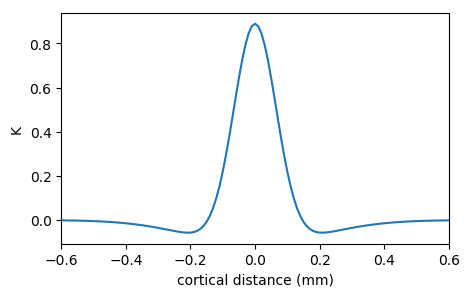
\includegraphics[width = 1.0\linewidth, trim={0 0 0 0}, clip=true]{figures/plot_K.png}
		\subcaption{$K_{aa'}$ where $a$ has been fixed a position $0$ and $a'$ varies from $-0.6$mm to $0.6$mm.}
		\label{fig:plotK}	
	\end{subfigure}%
	\hspace{0.05\linewidth}
	\begin{subfigure}[t]{0.45\linewidth}
		\centering
		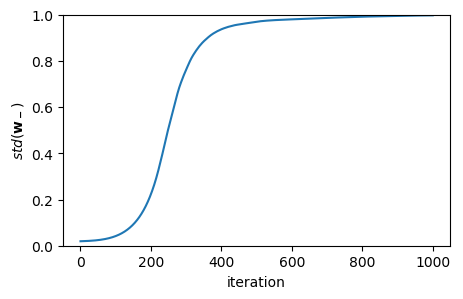
\includegraphics[width = 1.0\linewidth, trim={0 0 0 0}, clip=true]{figures/occsimtemp_stds.png}
		\subcaption{Standard deviation of ${\bf w}_-$ over time illustrating how ${\bf w}_-$ progresses from $\approx \bf 0$ to a vector of $ \pm 1$ after 800-1000 iterations.}
		\label{fig:stds}	
	\end{subfigure}%
\caption{}
\label{}
\end{figure}

We can also extract the vector ${\bf w}_-$ at different points in the simulation and plot the vector as a 1-dimensional heatmap along the x-direction where individual neurons are coloured from white to black according their ocular dominance (figure \ref{fig:occsim_int}).


\begin{figure}[h]
	\centering
	\begin{subfigure}[t]{0.60\linewidth}
		\centering
		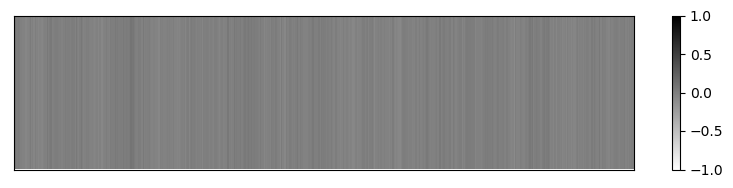
\includegraphics[width = 1.0\linewidth, trim={0 0 0 0}, clip=true]{figures/occsim_int/i50.png}
		%\subcaption{}
		%\label{fig:sim1vec}	
	\end{subfigure}%
	\hspace{0.03\linewidth}
	\begin{subfigure}[t]{0.60\linewidth}
		\centering
		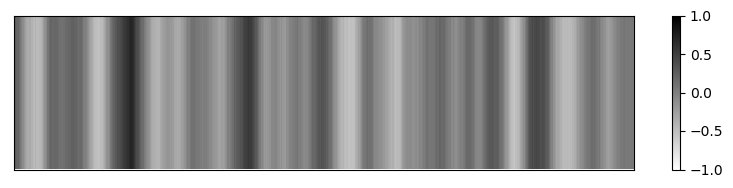
\includegraphics[width = 1.0\linewidth, trim={0 0 0 0}, clip=true]{figures/occsim_int/i200.png}
		%\subcaption{}
		%\label{fig:sim2vec}	
	\end{subfigure}%
	\hspace{0.03\linewidth}
	\begin{subfigure}[t]{0.60\linewidth}
		\centering
		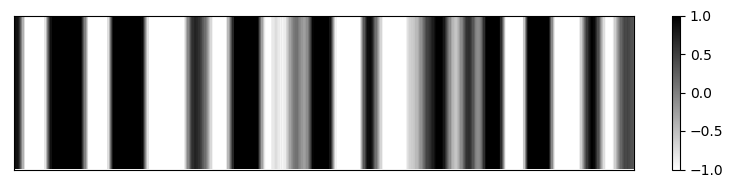
\includegraphics[width = 1.0\linewidth, trim={0 0 0 0}, clip=true]{figures/occsim_int/i300.png}
		%\subcaption{}
		%\label{fig:sim3vec}	
	\end{subfigure}%
	\hspace{0.03\linewidth}
	\begin{subfigure}[t]{0.60\linewidth}
		\centering
		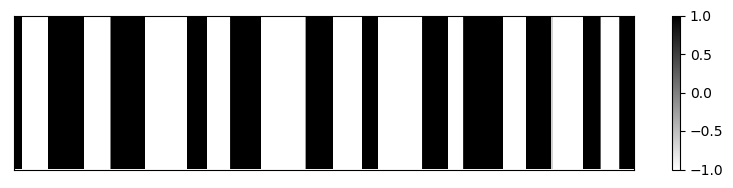
\includegraphics[width = 1.0\linewidth, trim={0 0 0 0}, clip=true]{figures/occsim_int/i1000.png}
		%\subcaption{}
		%\label{fig:sim3vec}	
	\end{subfigure}%
\caption{${\bf w}_-$ as a heatmap after 50, 200, 300 and 1000 iterations. We see that ocular dominance becomes increasingly strong over time and that the short-range excitation with long-range inhibition drives the formation of an oscillatory pattern of dominance.}
\label{fig:occsim_int}
\end{figure}

From our previous considerations, we expect the long-term behavior of ${\bf w}_-$ to be dominated by the prinpical eigenvector of $\bf K$.
In the case of periodic boundary conditions as imposed here, the eigenvectors of \textbf{K} are given by
\begin{equation}
e_a^\mu = \cos{(\dfrac{2 \pi \mu a}{512}-\phi)}
\end{equation}
Where $\mu = \dfrac{512 \cdot d \cdot k}{2 \pi}$ takes integer values and the eigenvalues are given by the discrete fourier transform $\tilde K(\mu) $.

Here, $k$ is the spatial frequency of the ocular dominance columns and $d$ is the separation between sites $a$ and $a+1$; i.e. $d = \dfrac{10 mm}{512}$. The principal eigenvector is thus the eigenfunction $e_\mu$ with $\mu$ corresponding to the maximum of $\tilde K(\mu)$, the discrete fourier transform of \textbf{K}.

To find the principal eigenvector of \textbf{K} and thus the expected long-term behavior of the system, we first find $\tilde K(k)$.
\begin{equation}
\tilde K (k) = \int_{-\infty}^\infty{K(x) e^{-2 \pi i k x} dx }
\end{equation}

We know that the fourier transform is a linear operator and that the fourier transform of a gaussian is given by
\begin{equation}
G(k) = \int_{-\infty}^\infty{ \dfrac{1}{\sqrt{2 \pi \sigma^2}} \, e^{\dfrac{-x^2}{2 \sigma^2}} e^{-2 \pi i k x} dx } 
= e^{\dfrac{-k^2 \sigma^2}{2}}
\end{equation}

This allows us to easily calculate the required fourier transform
\begin{equation}
\tilde K(k) = \sqrt{2 \pi \sigma^2} e^{ \dfrac{- k^2 \sigma^2}{2} } - \dfrac{1}{9} \sqrt{18 \pi \sigma^2 } e^{\dfrac{-9 k^2 \sigma^2}{2}}
\end{equation}
We plot this in figure \ref{fig:Ktilde} and find that the maximum of $\tilde K = 0.128$ occurs at $k = 8.17$. We can now find the value of $\mu$ corresponding to this maximum $\tilde K$ as
\begin{equation}
\mu_{max} = \dfrac{512 \,\,\, 8.17}{2 \pi} \dfrac{10}{512} = 13
\end{equation}
This allows us to calculate the principal eigenvector $e_{\mu_{max}}$ as a function of cortical distance and we plot this in figure \ref{fig:eigvec}. We note that the pattern of inhibition and excitation follows that of $K$ in figure \ref{fig:plotK}.
Since $\mu_{max}=13$, we expect to generate 13 periods of left and right dominance in our system in a given simulation which is consistent with the results in figure \ref{fig:occsim_int}. 

\begin{figure}[h]
	\centering
	\begin{subfigure}[t]{0.45\linewidth}
		\centering
		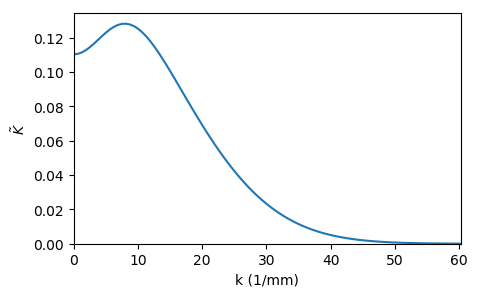
\includegraphics[width = 1.0\linewidth, trim={0 0 0 0}, clip=true]{figures/plot_Ktilde.png}
		\subcaption{Fourier transform of K as a function of spatial frequency $k$. This has a maximum of $k=8.17$ corresponding to $\mu=13$ suggesting that we will generate 13 periods of ocular dominance in a simulation with these parameters.}
		\label{fig:Ktilde}	
	\end{subfigure}%
	\hspace{0.05\linewidth}
	\begin{subfigure}[t]{0.45\linewidth}
		\centering
		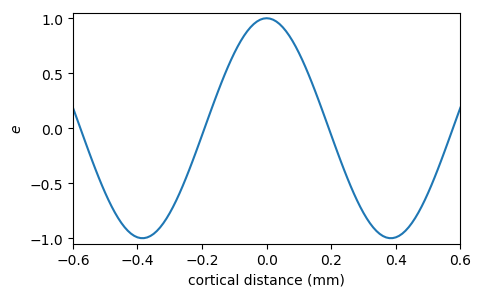
\includegraphics[width = 1.0\linewidth, trim={0 0 0 0}, clip=true]{figures/plot_eigvec.png}
		\subcaption{Principal eigenvector of K capturing the pattern of short-range excitation and long-range inhibition.}
		\label{fig:eigvec}	
	\end{subfigure}%
\caption{}
\label{}
\end{figure}

We now repeat our simulation of the system 1000 times and calculate the magnitude of the discrete fourier transform (DFT) at each trial. We plot the mean of the DFTs in figure \ref{fig:DFT} and see that the major components of our equilibrium ${\bf w}_-$ vector do indeed correspond to the values of $k$ for which $\tilde K$ is highest in figure \ref{fig:Ktilde}. 

\begin{figure}[h]
	\centering
	\begin{subfigure}[t]{0.45\linewidth}
		\centering
		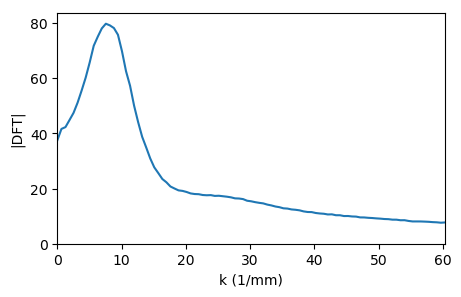
\includegraphics[width = 1.0\linewidth, trim={0 0 0 0}, clip=true]{figures/plot_DFT.png}
		\subcaption{Mean magnitude of the discrete fourier transform of the steady state ${\bf w}_-$ vector across 1000 simulations.}
		\label{fig:DFT}	
	\end{subfigure}%
	\begin{subfigure}[t]{0.45\linewidth}
		\centering
		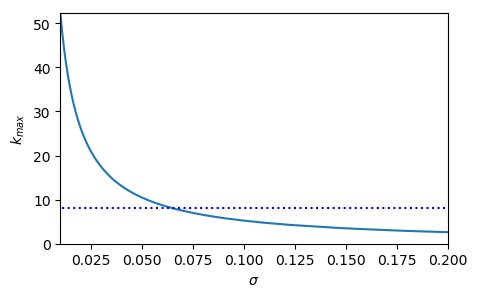
\includegraphics[width = 1.0\linewidth, trim={0 0 0 0}, clip=true]{figures/test_maxk.png}
		\subcaption{Principal eigenvector of \textbf{K}}
		\label{fig:maxk}	
	\end{subfigure}%
\caption{}
\label{}
\end{figure}

We find that the mean of the DFTs has a maximum of $79.7$ at $\mu = 13$ which is consistent with our analytical considerations suggesting that the largest component of the long-time ${\bf w}_-$ vector should correspond to the principal eigenvector which does indeed have $\mu = 13$

The stripe width in this model is determined by the spatial range of excitatory and inhibitory interactions which in turn is specified by the scale parameter $\sigma$ in equation \ref{eq:cortint}.
In order to decrease the stripe width in the model, we need to decrease the scale parameter $\sigma$ which leads to an increase in the value of $k$ that maximizes our discrete fourier transform and thus an increased frequency of the principal eigenvector of $\bf K$. In order to increase the stripe width, we instead increase $\sigma$.

The relationship between $\sigma$ and $k$ has been investigated numerically, and the value of $k$ that maximizes $\tilde K$ for a given $\sigma$ has been plotted in figure \ref{fig:maxk} which shows a rapid increase in frequency as $\sigma \rightarrow 0$.

To validate these results, we run two additional simulations; one with $\sigma = 0.012$ for which we expect $k=40.31$ and thus $\mu = 69$, and one with $\sigma=0.174$ for which we expect $k=3.01$ and $\mu = 5$. We plot the resulting steady state ${\bf w}_-$ vectors in figure \ref{fig:sigs} and see that we do indeed get increasingly wider stripes with increasing $\sigma$ and that the number of full periods matches the expected value of $\mu$.

\begin{figure}[h]
	\centering
	\begin{subfigure}[t]{0.60\linewidth}
		\centering
		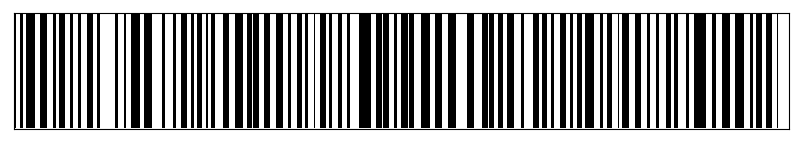
\includegraphics[width = 1.0\linewidth, trim={0 0 0 0}, clip=true]{figures/occsim_012_heat.png}
		\subcaption{$\sigma = 0.012$ giving $k=40.31$ and $\mu = 69$}
		%\label{fig:sim1vec}	
	\end{subfigure}%
	\hspace{0.03\linewidth}
	\begin{subfigure}[t]{0.60\linewidth}
		\centering
		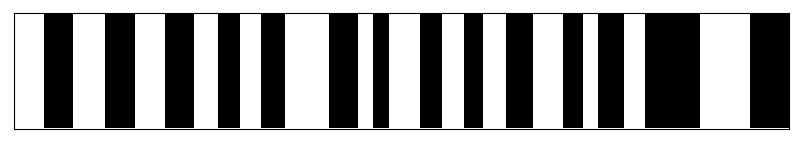
\includegraphics[width = 1.0\linewidth, trim={0 0 0 0}, clip=true]{figures/occsim_066_heat.png}
		\subcaption{$\sigma = 0.066$ giving $k=8.17$ and $\mu = 13$}
		%\label{fig:sim2vec}	
	\end{subfigure}%
	\hspace{0.03\linewidth}
	\begin{subfigure}[t]{0.60\linewidth}
		\centering
		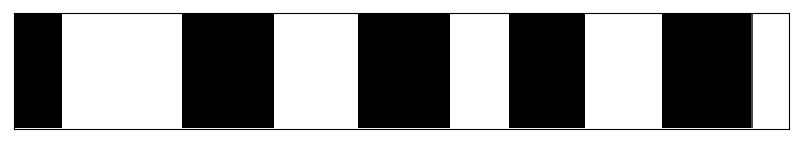
\includegraphics[width = 1.0\linewidth, trim={0 0 0 0}, clip=true]{figures/occsim_174_heat.png}
		\subcaption{$\sigma=0.174$ giving $k=3.01$ and $\mu = 5$}
		%\label{fig:sim3vec}	
	\end{subfigure}%
\caption{Simulations of the ocular dominance system for different values of $\sigma$ corresponding to different interaction ranges. Longer-range interactions lead to wider stripes.}
\label{fig:sigs}
\end{figure}

We could of course also alter the cortical interactions in other ways, e.g. by altering the ratio of the two gaussians from $1 : \dfrac{1}{9}$ or by changing the relative standard deviations from $\sigma_2 = 3 \sigma_1$, but these options are not explored further as they do not preserve the form of the interactions.

\section{The elastic net}

The Travelling salesman problem is an example of an NP complete problem, and there is thus no (current) algorithm that can solve it in polynomial time. As the number of nodes to be visited N increases, we are therefore forced to use various heuristic algorithms to try to approximate optimal solutions. One such algorithm dubbed the 'elastic net' was implemented by Durbin and Willshaw in a 1987 letter to \textit{Nature}.

In this algorithm, there are N cities to be visited, and this is achieved by distorting an initial path of M points until it runs through all N cities in a way that locally minimizes the path length L.
We denote the cities to be visited $\{x_i\}$ and the M points on the path travelled on $\{y_j\}$. At each timepoint the elastic net then updates each point on the path according to
\begin{equation}\label{eq:update}
\Delta y_j =\alpha \sum_i{w_{ij}(x_i-y_j) + \beta K (y_{j+1} - 2y_j + y_{j-1})} 
\end{equation}

The first term serves to decrease the distance between a point on the path and a city, ensuring that all points on the path will eventually run through a city. The second term serves to bring the points as close to each other as possible, ensuring that the path length is minimized.

In equation \ref{eq:update}, the weights $w_{ij}$ are given by
\begin{equation}
w_{ij} = \dfrac{\phi(|x_i-y_j|, K)}{\sum_k{\phi(|x_i-y_k|, K)}}
\end{equation}
Where
\begin{equation}
\phi (d, K) = \exp{(\dfrac{-d^2}{2K^2})}
\end{equation}
This implementation of the elastic net corresponds to minimizing an energy function
\begin{equation}\label{eq:energy}
E = -\alpha K (\sum_i{\ln{\sum_j{\phi(|x_i-y_j|, K)}}})+\beta \sum_j{|y_{j+1}-y_j|^2}
\end{equation}
Where again the first term penalizes when the path is far from a city and the second term penalizes a long path.
Our update step from equation \ref{eq:update} then has the property
\begin{equation}
\Delta y_j = -K \dfrac{\partial E}{\partial y_j}
\end{equation}
We are thus carrying out gradient descent on equation \ref{eq:energy} with adaptive learning rate K, ensuring that we will eventually arrive at a local minimum of the energy.

Over the course of the optimization, Durbin and Willshaw reduce K by 1\% every 25 iterations from $K=0.2$ to $K=0.01$ and fix $M = 2.5N$. However, given the advances in computing power since 1987, we can explore the effect of K and M on the performance of the algorithm more thoroughly.

For the remainder of this section we set $\alpha = 0.2$ and $\beta = 2.0$ as in Durbin and Willshaw, and we choose points on our initial path to be evenly spread out at a distance $0.1+\text{unif}(-0.001, 0.001)$ from the centroid of the cities. Cities are generated as a grid of 100 randomly distributed points in a 1x1 square.

We let K decay exponentially according to $K = 0.2*\exp{-\lambda n}$ where n is the number of timesteps, and a simulation is considered finished when $K < 0.001$. We can now vary lambda and the number of points M on our path to optimize the TSP optimization with the result of a coarse-grained parameter grid given in figure \ref{fig:tspopt}.  

\begin{figure}[h]
	\centering
	\begin{subfigure}[t]{0.35\linewidth}
		\centering
		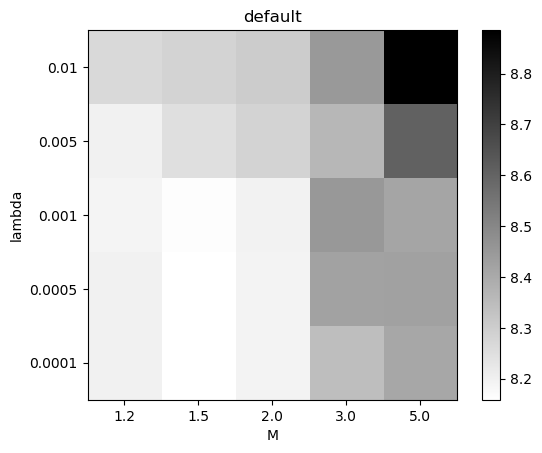
\includegraphics[width = 1.0\linewidth, trim={8 10 7 20}, clip=true]{figures/Ls.png}
		\subcaption{Length of final path}
		\label{fig:Ls}	
	\end{subfigure}%
	\hspace{0.1\linewidth}
	\begin{subfigure}[t]{0.35\linewidth}
		\centering
		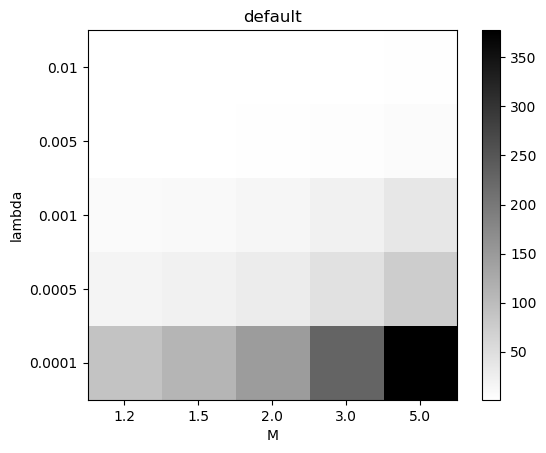
\includegraphics[width = 1.0\linewidth, trim={8 10 7 20}, clip=true]{figures/Ts.png}
		\subcaption{Time to convergence (seconds)}
		\label{fig:Ts}	
	\end{subfigure}%
\caption{Performance and computational time for the elastic net approach to the travelling salesman problem as a function of decay rate $\lambda$ and number of points on the path M. All simulations were run on the same set of 100 cities with remaining parameters as specified in the main text.}
\label{fig:tspopt}
\end{figure}

We see from figure \ref{fig:Ls} that in contrast to the parameters used by Durbin and Willshaw, we actually ahieve the best performance with a relatively small value of M=1.5N since small values of M tend to reduce the popensity of the system to get caught in higher-energy local minima compared to $M > 2N$. We also note that there is an increase in performance with decreasing lambda as expected, but this effect is neglible for $\lambda < 0.0005$.

From figure \ref{fig:Ts} we see that the time taken for a simulation is approximately linear in both $\lambda$ and M. Considering this data together with figure \ref{fig:Ls}, we therefore pick M=1.5 and $\lambda = 0.0005$ for the remainder of our simulations. More finegrained optimization could be carried out, but this was not deemed particularly informative since the details of the optimization will depend upon the specific grid being investigated. However, the above analysis was repeated with two additional random grids and similar patterns were observed.

We can now investigate how the path develops as K decreases for our optimum parameters of M=1.5 and $\lambda = 0.0005$ (figure \ref{fig:tspsim}). We see that the path initially expands relatively uniformly to decrease the distance from the far-away cities to the path. The path then locally distorts as it moves closer to every individual point. This is finally achieved at K=0.001 where the path has converged and the salesman visits every city. When M gets too close to N, the algorithm occasionally converges to a local minimum where the path does not visit every city. For $M \geq 1.5N$ this has not been observed.

\begin{figure}[h]
	\centering
	\begin{subfigure}[t]{0.24\linewidth}
		\centering
		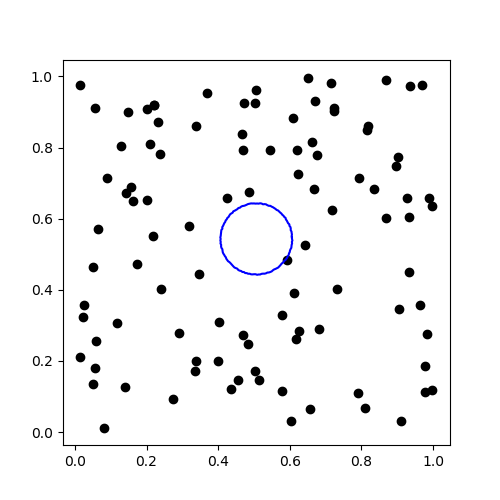
\includegraphics[width = 1.0\linewidth, trim={20 20 30 30}, clip=true]{figures/optimum_1.png}
		\subcaption{K=0.2}
		\label{fig:sim1}	
	\end{subfigure}%
	%\hspace{0.01\linewidth}
	\begin{subfigure}[t]{0.24\linewidth}
		\centering
		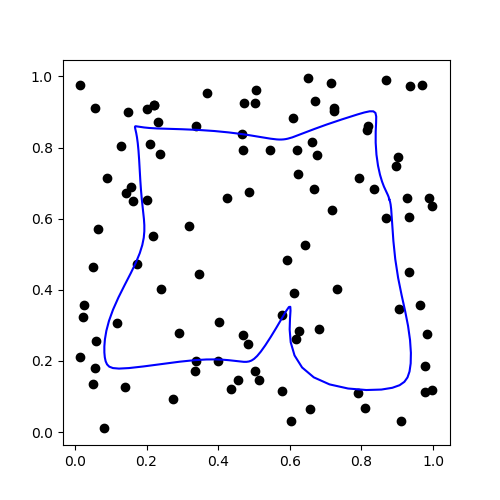
\includegraphics[width = 1.0\linewidth, trim={20 20 30 30}, clip=true]{figures/int/optimum_K6_011.png}
		\subcaption{K=0.11}
		\label{fig:sim2}	
	\end{subfigure}%
	%\hspace{0.01\linewidth}
	\begin{subfigure}[t]{0.24\linewidth}
		\centering
		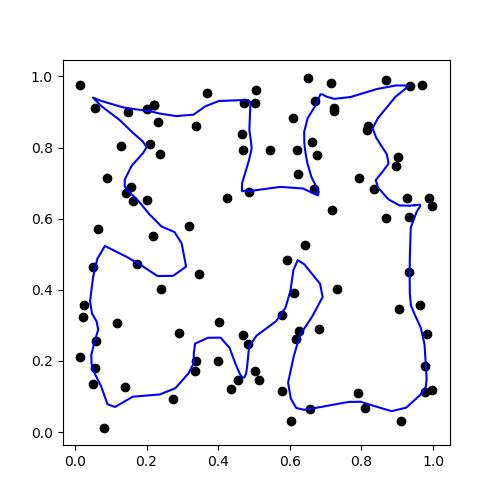
\includegraphics[width = 1.0\linewidth, trim={20 20 30 30}, clip=true]{figures/int/optimum_K16_004.png}
		\subcaption{K=0.04}
		\label{fig:sim3}	
	\end{subfigure}%
	%\hspace{0.01\linewidth}
	\begin{subfigure}[t]{0.24\linewidth}
		\centering
		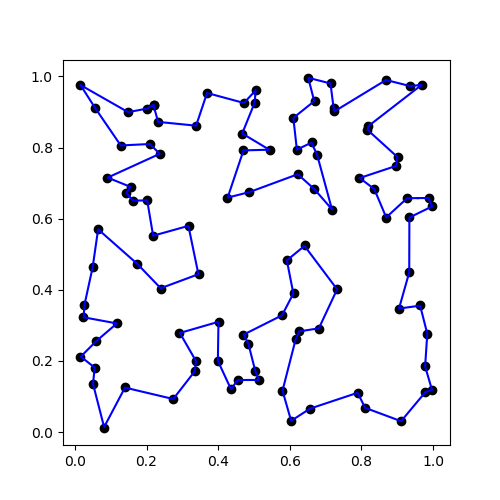
\includegraphics[width = 1.0\linewidth, trim={20 20 30 30}, clip=true]{figures/optimum_2.png}
		\subcaption{K=0.001}
		\label{fig:sim4}	
	\end{subfigure}%
\caption{Timecourse of the travelling salesman simulation with M=1.5 and $\lambda = 0.0005$}
\label{fig:tspsim}
\end{figure}

At a first glance, this looks like a reasonable route as there are no obvious detours or crossovers. However, to get a better idea of how efficient the elastic net method is, we can compare it with the well established travelling salesman method of simulated annealing. For this comparison, we implement simulated annealing as described in \textit{Stochastic Processes} (Chang 2007).

We can consider a given TSP route (order of cities) to be a point in a set $\mathcal{S}$ of $\dfrac{(n-1)!}{2}$ possible routes. Our aim is to find a route that minimizes the total length $L$ by moving between neighboring points on $\mathcal{S}$. Here, we define 'neighboring points' as routes that can be interconverted by reversing the part of the path between two cities.

In the simulated annealing algorithm, one iteration involves moving uniformly at random to a neighboring point in $\mathcal{S}$ and calculating the length $L1$ of the new route obtained.
If $L1 < L0$, we accept this new route as our current route.
If $L1 > L0$, we accept the new route with probability $p = \exp{(-\dfrac{L1-L0}{T})}$. Otherwise we retain the old route.

This finite probability of accepting a worse route allows us to move out of local minima and thus to approach the global minimum with a higher probability than a simple gradient descent algorithm. This is similar to e.g. the annealing process in glass (from which the algorithm has its name), or protein folding in a cell where the finite temperature allows for stochastic movement out of local minima in conformational space.

Over the course of the simulation, we decrease the tempeature according to 
\begin{equation}
T_n = \dfrac{T_0}{ln(n)}
\end{equation}
Here n is the number of iterations. The decrease in temperature makes it increasingly unlikely that we will move to a worse route, and in the limit of $T \rightarrow 0$, we will move to the nearest local minimum as there is no thermal energy in the system to drive it to a longer path.

Setting $T_0=10$ and running $10^7$ iterations has been found empirically to give good results on a timescale similar to the one observed for the elastic net (\~ 20 seconds).
To compare the two methods, we use the map of 100 cities considered above as well as two new randomly generated maps. We then quantify the optimum route generated by the elastic net in terms of both route length and time to convergence. We compare this to 30 trials of simulated annealing since the simulated annealing process is stochastic and results thus vary per trial. A summary of the results is given in table \ref{tab:tsp}.

\begin{table}[h]
\centering
\begin{tabular}{ |c|c|c|c|}
\hline
 &Map 1 &Map 2 & Map 3 \\
\hline
Elastic net & 8.159 & 7.771 & 7.815 \\
Time (s) & 23.32 & 23.819& 24.91 \\
\hline
Simulated annealing & 7.956 (0.047) & 7.768 (0.052)& 7.633 (0.075)\\
Time (s) & 19.06 (1.33) & 19.47 (1.97) & 18.47 (1.12)\\
\hline
\end{tabular}
\caption{Performance and computational time for the elastic net and simulated annealing across three different maps of 100 randomly generated cities. For simulated annealing, the numbers in brackets represent standard deviations from 30 trials.}
\label{tab:tsp}
\end{table}

We see that simulated annealing consistently outperforms the elastic net, both in terms of the converged route and the time taken to find this route. This can be seen qualitatively in figure \ref{fig:comp1}.

\begin{figure}[h]
	\centering
	\begin{subfigure}[t]{0.28\linewidth}
		\centering
		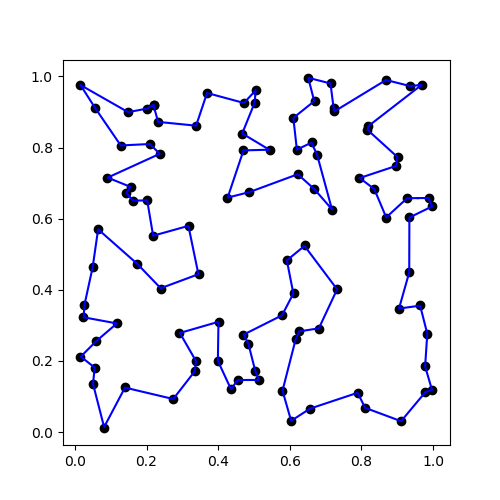
\includegraphics[width = 1.0\linewidth, trim={20 20 30 30}, clip=true]{figures/optimum_2.png}
		\subcaption{Elastic net (L=8.159)}
		\label{fig:comp1el}	
	\end{subfigure}%
	\hspace{0.1\linewidth}
	\begin{subfigure}[t]{0.28\linewidth}
		\centering
		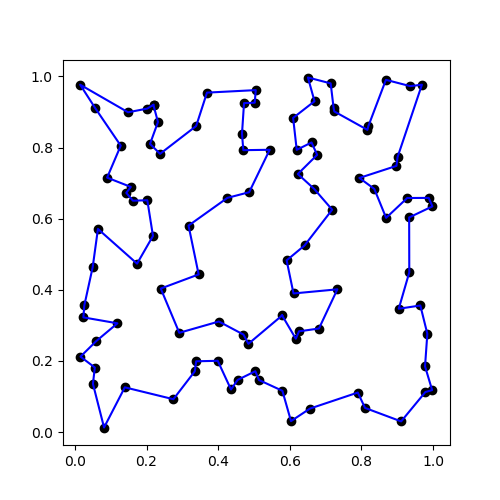
\includegraphics[width = 1.0\linewidth, trim={20 20 30 30}, clip=true]{figures/orig_citiesmin.png}
		\subcaption{Simulated annealing (L = 7.919)}
		\label{fig:comp1an}	
	\end{subfigure}%
\caption{Optimum routes for map 1 found by the elastic net method and simulated annealing. Simulated annealing finds a shorter route than the elastic net, and this route involves only visiting the inner region of the map once. }
\label{fig:comp1}
\end{figure}

However, for map 2 simulated annealing only slightly outperforms the elastic net and performs worse for half the trials, raising the question of whether there are any profound insights to be gained from this difference between maps. For map 1, we find that the optimum route from simulated annealing appears very asymmetric. It is thus less likely to be converged upon by the elastic net, the dynamics of which lead to an initial expansion of the route followed by the formation of local invaginations (figure \ref{tspsim}).

For map 2, on the contrary, the optimum route from simulated annealing appears more symmetrical which might explain why the elastic net comes close to the performance of simulated annealing in this case.


\begin{figure}
	%\hspace{0.31\linewidth}
	\centering
	\begin{subfigure}[t]{0.28\linewidth}
		\centering
		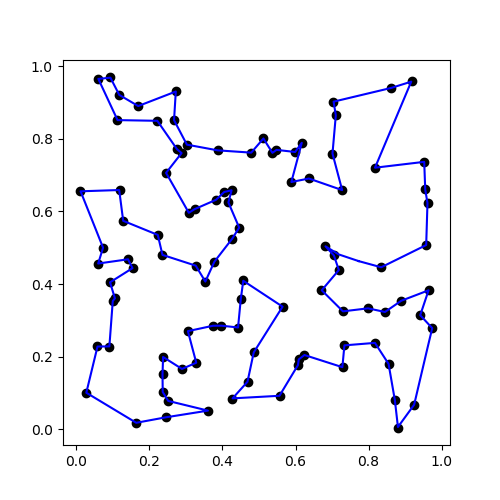
\includegraphics[width = 1.0\linewidth, trim={20 20 30 30}, clip=true]{figures/rand1_2.png}
		\subcaption{Elastic net (L = 7.771)}
		\label{fig:comp2el}	
	\end{subfigure}%
	\hspace{0.1\linewidth}
	\begin{subfigure}[t]{0.28\linewidth}
		\centering
		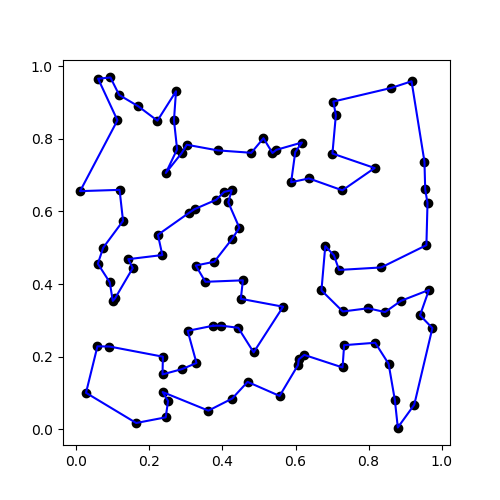
\includegraphics[width = 1.0\linewidth, trim={20 20 30 30}, clip=true]{figures/rand1_citiesmin.png}
		\subcaption{Simulated annealing (L = 7.685)}
		\label{fig:comp2an}	
	\end{subfigure}%
\caption{For map 2, the solutions found by simulated annealing are more symmetrical, and the elastic net comes close to the performance of simulated annealing.}
\label{fig:comp2}
\end{figure}


Simulated annealing is thus a superior method to the elastic net in terms of solving the travelling salesman problem, but we see that the elastic net still produces reasonable routes that are comparable in length to those generated by simulated annealing albeit generally more symmetric. The elastic net methodology is therefore still somewhat interesting due to its different dynamics and blah blah...

To use the elastic net to model ocular dominance in 2 dimensions, we imagine the tour as being a plane representing a region of the visual cortex. Each point has elastic connections to each other point. The retinal input are represented by two horizontal planes corresponding to the left and right eyes respectively with each point being the equivalent of a city in the TSP. We now index our tour with $i, j$ and the retinal positions by $a, b$. This gives a new 20

\begin{equation}\label{eq:update}
\Delta y_{ij} =\alpha \sum_{a,b}{w_{ab,ij}(x_{ab}-y_{ij})} + \beta K (y_{i \, j+1} + y_{i+1 \, j} - 4y_{i \, j} + y_{i \, j-1} + y_{i-1 \, j}
\end{equation}


\section{Cart pole balancing problem}

\textit{Associate Search Element} (ASE). Picks a decision based on a reward signal and eligibility trace.
\textit{Adaptive Critic Element} (ACE) provides the ASE with a predicted reward over continuous time rather than a discrete reward at the end of a trial.

State of the cartpole balancing problem defined by a vector $(x, \theta, \dot x, \dot \theta)$ where $x$ is the position of the cart on a one-dimensional track with $x \in [-2.4, 2.4]$.
$\theta$ is the angle of the pole from vertical and dots represent time derivatives. A trial is considered to have failed when $|x| \geq 2.4$ or $| \theta | \geq 12 \degree$.

We divide the state space into 162 distinct regions defined by\\
$x \in [-2.4,-0.8], [-0.8,0.8],[0.8,2.4]$ m\\
$\theta \in [-12,-6],[-6,-1],[-1,0],[0,1],[1,6],[6,12]$ $\degree$\\
$\dot x \in [-\infty,-0.5],[-0.5,0.5],[0.5,\infty]$ m/s\\
$\dot \theta \in [-\infty,-50],[-50,50],[50,\infty]$ $\degree$/s\\

At any time t, the system will be in a given state $state(t)$ and it receives an impulse either to the right or to the left based on the relative predicted reward for right and leftwards impulses for as represented by $w_i(t)$ for state i. We therefore map a given state vector to a binary 162-dimensional vector that has all elements equal to zero except for the element corresponding to the current state of the system.

The output of an element is then determined by
\begin{equation}
y(t) = \text{sign}[\sum_i^{162}{w_i(t)x_i(t)} + \mathcal{N}(0, \sigma^2)] = \text{sign}[w_{state(t)}(t) + \mathcal{N}(0, \sigma^2)] 
\end{equation}

Where $x_i(t)$ is $1$ if the system is in state $i$ at time $t$ and zero otherwise, and $w_{state(t)}(t)$ is the weight at time t corresponding to the state of the system at time t. The Gaussian noise both simulates noise in real neural systems and allows our cart pole balancing system to explore the available state space.

For the ASE we update the weights according to
\begin{equation}
w_i(t+1) = w_i(t) + \alpha r(t) e_i(t)
\end{equation}
This is a three-factor learning rule where $\alpha$ is the learning rate, $r(t)$ is the global reward at time $t$ and $e_i(t)$ is the eligibility trace of unit $i$ at time $t$. For the pole balancing problem, $r=0$ throughout a trial and becomes $1$ when failure occurs. We update the eligiblity traces according to

\begin{equation}
e_i(t+1) = \delta e_i(t) + (1-\delta) y(t) x_i(t)
\end{equation}
where $\delta$ determines the trace decay rate and $x, y$ are as defined above.

This system does not perform particularly well given the sparse error signal which only occurs after a long sequence of events. Performance is better if we include an ACE which estimates a predicted error at all times.
The predicted error is given by
\begin{equation}
\hat r(t) = r(t) + \gamma p(t) - p(t-1)
\end{equation}
Here, $\gamma$ leads to the predicted reward tending towards 0 in the case of prolonged periods without external reinforcement.
$p(t)$ is a prediction of eventual reinforcement, given by
\begin{equation}
p(t) = \sum_i^{162}{v_i(t)x_i(t) = v_{state(t)}(t)}
\end{equation}
This requires us to update the weights $v_i$ such that they remain an accurate predictor of reward. This is achieved using the learning rule
\begin{equation}
v_i(t+1) = v_i(t) + \beta[r(t) + \gamma p(t) - p(t-1)] \bar x_i(t)
\end{equation}
Here, $\beta$ determines the learning rate and $r(t)$ is the external reinforcement signal as above. $\bar x_i(t)$ is similar to the eligibility trace $e_i(t)$ for the ASE and is updated according to
\begin{equation}
\bar x_i(t+1) = \lambda \bar x_i(t) + (1-\lambda)x_i(t) 
\end{equation}
Where $\lambda$ is the trace decay rate. This is equivalent to the update rule for $e_i(t)$ with $y_i(t) = 1$.


We initialize all $e_i, w_i, v_i = 0$ at time $t=0$.
We intialize the cart at x=0 and the pole at an angle of 0 degrees. the first impulse is thus stochastic and determined entirely by the noise term.

Brato et al. using Euler integration with a timestep of 0.02 seconds in the original paper. However, we find this to give highly inaccurate intergration and instead use a timestep of 0.001

$\alpha = 1000$
$\beta = 0.5$
$\delta = 0.9$
$\gamma = 0.95$
$\lambda = 0.80$
$\sigma = 0.01$



Maintaining the cart within the bounds and maintaining the pole upright are of course related; for the default specs, the pole never falls over. However, we can shorten the pole half length to $0.1$m in which case the pole does fall over but the cart never reaches the bounds of the track. At 0.2, both can happen.

\begin{figure}[h]
	\centering
	\begin{subfigure}[t]{0.28\linewidth}
		\centering
		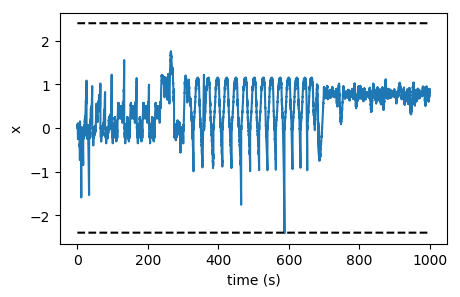
\includegraphics[width = 1.0\linewidth, trim={0 0 0 0}, clip=true]{figures/learn50000_xs.png}
		\subcaption{Elastic net (L=8.159)}
		\label{fig:comp1el}	
	\end{subfigure}%
	\hspace{0.1\linewidth}
	\begin{subfigure}[t]{0.28\linewidth}
		\centering
		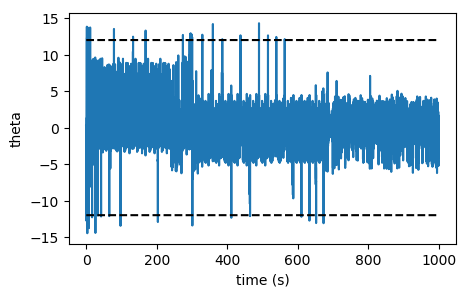
\includegraphics[width = 1.0\linewidth, trim={0 0 0 0}, clip=true]{figures/learn50000_thetas.png}
		\subcaption{Simulated annealing (L = 7.919)}
		\label{fig:comp1an}	
	\end{subfigure}%
\caption{Optimum routes for map 1 found by the elastic net method and simulated annealing. Simulated annealing finds a shorter route than the elastic net, and this route involves only visiting the inner region of the map once. }
\label{fig:comp1}
\end{figure}

Set l=0.1


\begin{figure}[h]
	\centering
	\begin{subfigure}[t]{0.28\linewidth}
		\centering
		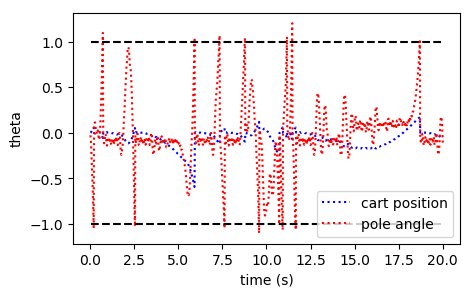
\includegraphics[width = 1.0\linewidth, trim={0 0 0 0}, clip=true]{figures/learn1000_xs_thetas.png}
		\subcaption{Elastic net (L=8.159)}
		\label{fig:comp1el}	
	\end{subfigure}%
	\hspace{0.1\linewidth}
	\begin{subfigure}[t]{0.28\linewidth}
		\centering
		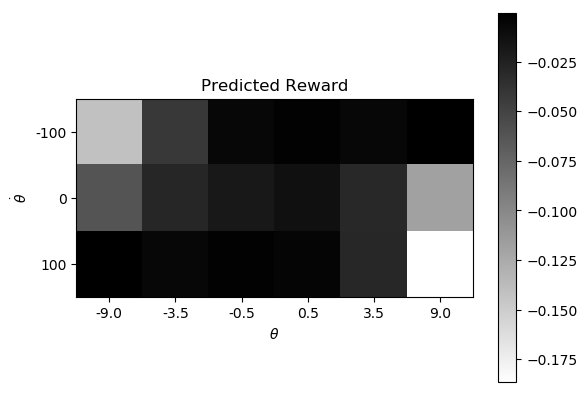
\includegraphics[width = 1.0\linewidth, trim={0 0 0 0}, clip=true]{figures/learnvs_vs.png}
		\subcaption{Simulated annealing (L = 7.919)}
		\label{fig:comp1an}	
	\end{subfigure}
\caption{Optimum routes for map 1 found by the elastic net method and simulated annealing. Simulated annealing finds a shorter route than the elastic net, and this route involves only visiting the inner region of the map once. }
\label{fig:comp1}
\end{figure}

\begin{figure}[h]
	\centering
	\begin{subfigure}[t]{0.28\linewidth}
		\centering
		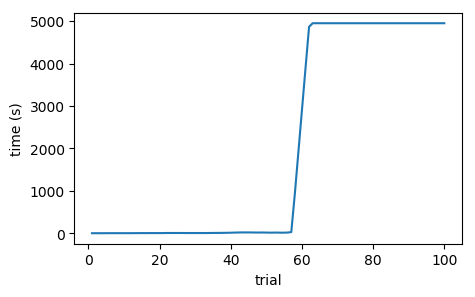
\includegraphics[width = 1.0\linewidth, trim={0 0 0 0}, clip=true]{figures/learn500000_performance.png}
		\subcaption{Elastic net (L=8.159)}
		\label{fig:comp1el}	
	\end{subfigure}%
	\hspace{0.1\linewidth}
	\begin{subfigure}[t]{0.28\linewidth}
		\centering
		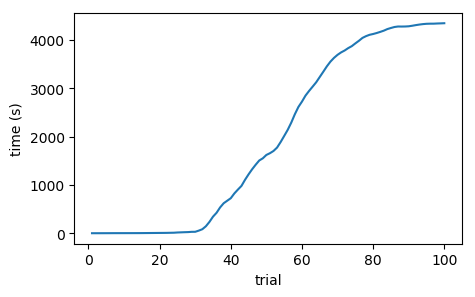
\includegraphics[width = 1.0\linewidth, trim={0 0 0 0}, clip=true]{figures/real_meanperformance.png}
		\subcaption{Simulated annealing (L = 7.919)}
		\label{fig:comp1an}	
	\end{subfigure}
\caption{Optimum routes for map 1 found by the elastic net method and simulated annealing. Simulated annealing finds a shorter route than the elastic net, and this route involves only visiting the inner region of the map once. }
\label{fig:comp1}
\end{figure}

\begin{figure}[h]
	\centering
	\begin{subfigure}[t]{0.28\linewidth}
		\centering
		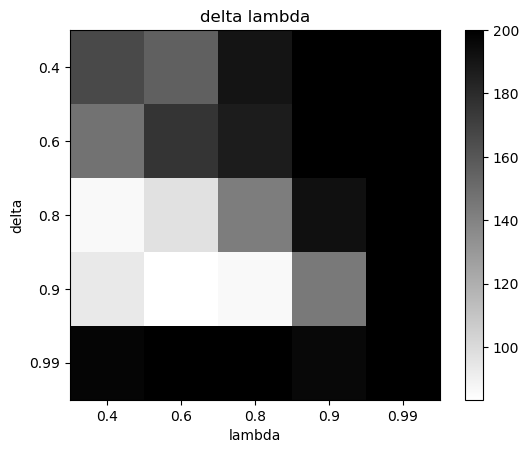
\includegraphics[width = 1.0\linewidth, trim={0 0 0 0}, clip=true]{figures/real_delta_lambda_heat.png}
		\subcaption{Elastic net (L=8.159)}
		\label{fig:comp1el}	
	\end{subfigure}%
	\hspace{0.1\linewidth}
	\begin{subfigure}[t]{0.28\linewidth}
		\centering
		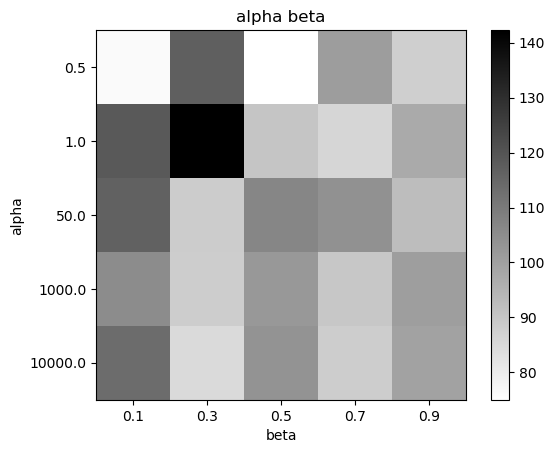
\includegraphics[width = 1.0\linewidth, trim={0 0 0 0}, clip=true]{figures/test_alpha_beta_heat.png}
		\subcaption{Simulated annealing (L = 7.919)}
		\label{fig:comp1an}	
	\end{subfigure}
	\begin{subfigure}[t]{0.28\linewidth}
		\centering
		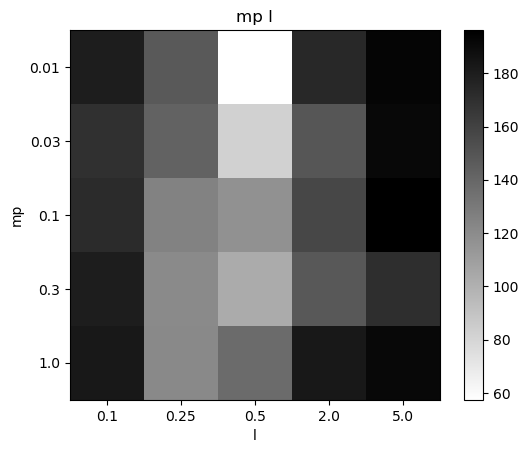
\includegraphics[width = 1.0\linewidth, trim={0 0 0 0}, clip=true]{figures/test_mp_l_heat.png}
		\subcaption{Simulated annealing (L = 7.919)}
		\label{fig:comp1an}	
	\end{subfigure}
\caption{Optimum routes for map 1 found by the elastic net method and simulated annealing. Simulated annealing finds a shorter route than the elastic net, and this route involves only visiting the inner region of the map once. }
\label{fig:comp1}
\end{figure}

lots of parameters in the model; won't vary all of them but will vary a few.

Eligibility trace ecay rates of the ASE and ACE (delta and lambda)
Length and mass of the pole
learnings rates (alpha and beta)
predicted reward decay rate (gamma)


We can add a second layer to the network and denote this z with weights from the input signal given by the matrix $D$

\begin{equation}
z_i(t) = g(\sum_{j=1}{D_{ij}(t) x_j(t)})
\end{equation}
Where $g(s) = \dfrac{1}{1+e^{-1}}$.

This allows us to calculate a probability
\begin{equation}
P_(t) = g(\sum_{i=1}{w_{i}(t) x_i(t)} + \sum_{i=1}{f_i(t)z_i(t)})
\end{equation}

where $f_i$ are the weights from the hidden layer to the output layer (equivalent to $w_i$ for the input layer).
We then have $y(t) = 1$ with probability $P(t)$ and $y(t) = -1$ with probability $1-P(t)$.

Our ACE also gets a hidden layer  $q$ with connectivity matrix $A$ from the input layer and activities
\begin{equation}
q_i(t) = g(\sum_{j=1}{A_{ij}(t) x_j(t)})
\end{equation}
\begin{equation}
p_(t) = \sum_{i=1}{v_{i}(t) x_i(t)} + \sum_{i=1}{c_i(t)q_i(t)}
\end{equation}

We then update weights according to

\begin{equation}
w_i(t+1) = w_i(t) + \alpha r(t)(\max{(y(t), 0)} - P(t))x_i(t)
\end{equation}
\begin{equation}
f_i(t+1) = f_i(t) + \alpha r(t)(\max{(y(t), 0)} - P(t))z_i(t)
\end{equation}
\begin{equation}
D_{ij}(t+1) = D_{ij}(t) + \alpha r(t) z_i(t) (1-z_i(t))\text{sign}(f_i(t)) (\max{(y(t), 0)} - P(t))x_j(t)
\end{equation}


\begin{equation}
v_i(t+1) = v_i(t) + \beta r(t) x_i(t)
\end{equation}
\begin{equation}
c_i(t+1) = c_i(t) + \beta r(t) q_i(t)
\end{equation}
\begin{equation}
A_{ij}(t+1) = A_{ij}(t) + \beta r(t) q_i(t) (1-q_i(t))\text{sign}(c_i(t)) x_j(t)
\end{equation}






in the present case, the additional layer does not significantly improve performance; however, Anderson had made the task more difficult by scaling, shifting and random initialization of the task and found that the second layer only improved performance after a large number of iterations. However, in the present simpler case, the network rapidly learns the task and the second layer is therefore not necessary.








\end{document}

